\chapter{Controlador de corriente} \chapterlabel{Informe/4-ControladorCorriente} \label{cap:ControladorCorriente}

En este capítulo se diseña y modela el circuito encargado de controlar la corriente que circula por el electroimán. Como se vio en el capítulo anterior, el sistema trabaja con corrientes elevadas por lo que se implementan estrategias de conmutación para reducir las pérdidas de energía. Para ello se utiliza una topología de puente H con cuatro MOSFET y un \textsl{driver} que los controla. Además, se detallan los criterios tenidos en cuenta al momento de  elegir  y dimensionar todos los componentes que intervienen para lograr el correcto funcionamiento del controlador de corriente. Por último, se obtiene su función transferencia  para ser utilizada en el diseño del compensador.

\section{Descripción general}

Para regular la fuerza electromagnética generada por el electroimán se debe modificar la intensidad de la corriente que circula por su bobinado. Para ello, es necesario diseñar una fuente de alimentación que permita proveer la corriente necesaria en cada momento para mantener en suspensión a la pieza móvil. 

Para diseñar la fuente de alimentación se debe conocer el comportamiento eléctrico de la planta. Como se analizó en el capítulo \ref{cap:CaracterizacionElectroiman}, el electroimán puede ser modelado como una inductancia variable con una resistencia serie. Es decir, es un circuito RL serie cuya corriente depende de la tensión aplicada y  se muestra en la expresión \ref{eq_corriente}.

\begin{equation} \label{eq_corriente}
	I_L=\frac{V_L}{sL(Y_g)\ +\ R_L}
\end{equation}


\noindent Se desea controlar la corriente que circula por el electroimán y, debido a que el sistema va a trabajar con corrientes elevadas, es importante que la implementación del controlador de corriente sea eficiente. Por lo tanto, para disminuir la disipación de potencia del circuito se utiliza un controlador que funciona en conmutación.

\colorbox{red}{lo escribiría como:}
Se desea entonces diseñar un circuito que le brinde al electroimán la alimentación adecuada para que por su bobinado circule una corriente contínua de un valor que pueda ser controlado de manera externa (mediante una tensión de referencia).

De la ecuación \ref{eq_admitancia} se puede observar que la corriente en el electroimán sufre un transitorio en forma de exponencial creciente para luego estabilizarse en un valor V/R en régimen permanente. La solución mas simple que se podría idear es la de utilizar un circuito que varíe la alimentación del electroimán. ¿como se logra esto? Si se tiene una fuente de alimentación fija para todo el circuito y se desea obtener una tensión variable en el bobinado, se podría implementar un circuito con un transistor funcionando en zona lineal y variar su tensión colector-emisor. \colorbox{red}{poner figura ejemplo}

Este circuito podría funcionar pero tiene la desventaja de que debido a que el sistema trabaja con corrientes elevadas se producen grandes pérdidas de energía en el transistor. 

Debido a que el sistema va a funcionar con corrientes elevadas, es importante minimizar las pérdidas de energía que puedan ocurrir en la circuitería del controlador de corriente. Por lo tanto, se debería implementar un controlador que trabaje en conmutación.  En este tipo de controladores se aprovecha el transitorio de corriente en el electroimán de manera que al alternar la polaridad de la tensión aplicada se puede hacer que la corriente crezca o decrezca alrededor de un valor medio. \colorbox{red}{cambiar figura}. Si se eligen tiempos de conmutación pequeños comparados con la constante de tiempo de la planta, la corriente tendrá una forma triangular.

\begin{figure}[H]
	\centering
	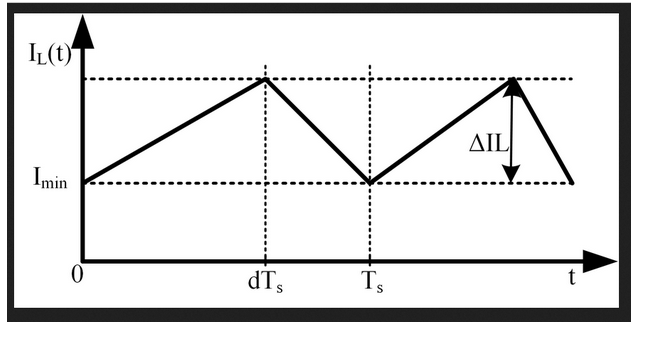
\includegraphics[scale=0.5]{triangular.png}
	\caption{Forma de onda de corriente.}
	\label{fig:img_corriente_triangular}
\end{figure}


\noindent Para lograr una corriente contínua en el electroimán mediante una fuente conmutada se debe alternar la polaridad de la tensión aplicada en los bornes del inductor. De esta forma, la corriente crece y decrece (según la polaridad de tensión aplicada) con forma exponencial debido a la resistencia interna del electroimán. Sin embargo, como el intervalo de tiempo de esta conmutación es pequeño comparado con la constante de tiempo de la planta, el incremento de corriente será pequeño y puede ser aproximado a una recta. Por lo tanto, se obtiene una corriente contínua con un ripple superpuesto de forma triangular, como la que se muestra en la figura \ref{fig:img_corriente_triangular_2}. 

\begin{figure}[H]
	\centering
	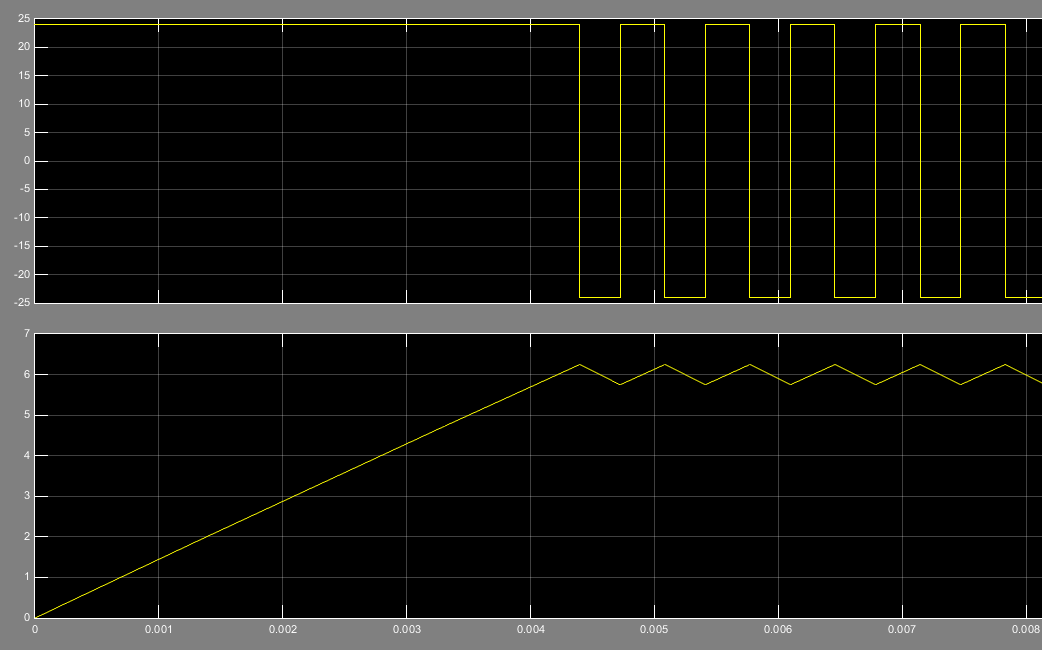
\includegraphics[scale=0.5]{corriente_triangular.PNG}
	\caption{Forma de onda de corriente.}
	\label{fig:img_corriente_triangular_2}
\end{figure}


\noindent Para lograr alternar la polaridad de la fuente sobre el inductor se utiliza una topología en puente H con cuatro llaves como se  muestra en la figura.

\begin{figure}[H]
	\centering
	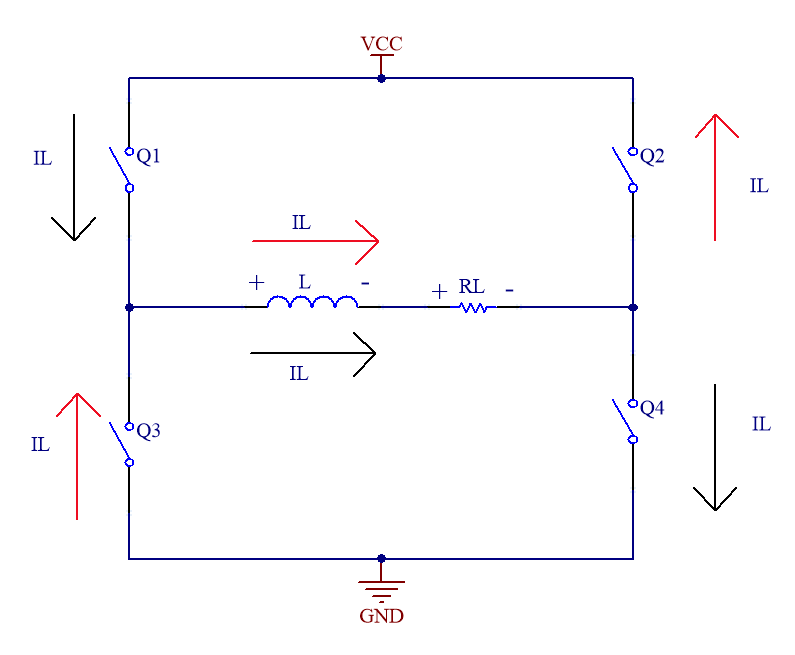
\includegraphics[scale=0.5]{puente_con_llaves.png}
	\caption{Topología simplificada.}
	\label{fig:img_topologia_simplificada}
\end{figure} 

El electroimán se conecta entre los puntos medios de cada par de llaves. De esta manera se puede conmutar la polaridad de la tensión que se le aplica. Sólo se permite que dos llaves se enciendan a la vez, y esto se realiza de manera diagonal. Es decir, en la figura \ref{fig:img_topologia-puenteH}, $Q_1$ y $Q_4$ pueden estar encendidos, mientras que $Q_3$ y $Q_2$ están apagados, y viceversa. De otra forma, se podría generar un cortocircuito entre la fuente de alimentación y GND, que produciría una circulación de corriente denominada \textsl{shoot-through}.

Para poder generar una corriente triangular con un valor medio deseado es necesario controlar el tiempo que se le aplica cierta polaridad de tensión al electroimán. Para poder controlar dicha polaridad, se debe actuar sobre las llaves en función de si se desea aumentar o disminuir el valor medio de la corriente.  Una manera de hacerlo es mediante un comparador con histéresis, cuya salida determina que llaves se encienden en función de comparar la corriente de referencia con la que está circulando por el electroimán. En caso de que esta última sea menor qeu la referencia, la polaridad de tensión aplicada al electroimán será positiva y, por ende, la corriente aumentara hasta alcanzar la referencia. Una vez superada la referencia, se volverá a cambiar la polaridad en el electoimán, pero esta vez será negativa, haciendo que el valor medio de la corriente disminuya. De esta forma, se puede observar que va a haber un riple en torno al valor medio de corriente deseado.  Este riple debe ser...



permanecen encendidas las llaves en 
Al controlar el tiempo de activación de las llaves, se podría obtener una forma de onda triangular con un valor medio determinado. Una manera de controlar las llaves es mediante un controlador con histéresis

La etapa de controlador de corriente tiene una tensiòn en su entrada que es tomada como referencia. Es decir, se desea que la corriente del electroimàn sea proporcional a esta tensiòn. Para ello primero se necesita medir la corriente que circula en el elctroimàn, traducirla a una tensiòn para luego esr comparada con esta referemcia. Dependiendo de si una es mayor que la otra, un controlador modifica el estado de las llaves para equiluibrar esta stiuacion. 

Es necesario poder controlar el comportamiento de las llaves para poder manejar cuándo la corriente en el inductor crece y decrece. 

Para poder determinar que llaves encender y cuales apagar, es necesario sabe saber si la corriente debe aumentar o disminuir.

Estas son controladas por un circuito que compara el valor de corriente con una referencia y conmuta las llaves segùn sea necesario.

 manejados por el controlador por histéresis como se observa en la figura \ref{fig:img_topologia-puenteH}. Pueden diferenciarse dos semiciclos de trabajo: uno de estado ON y otro de estado OFF. El primero se define como el semiciclo durante el cual la corriente en el inductor crece (pendiente positiva), mientras que el segundo se da cuando la corriente decrece.

\begin{figure}[H]
	\centering
	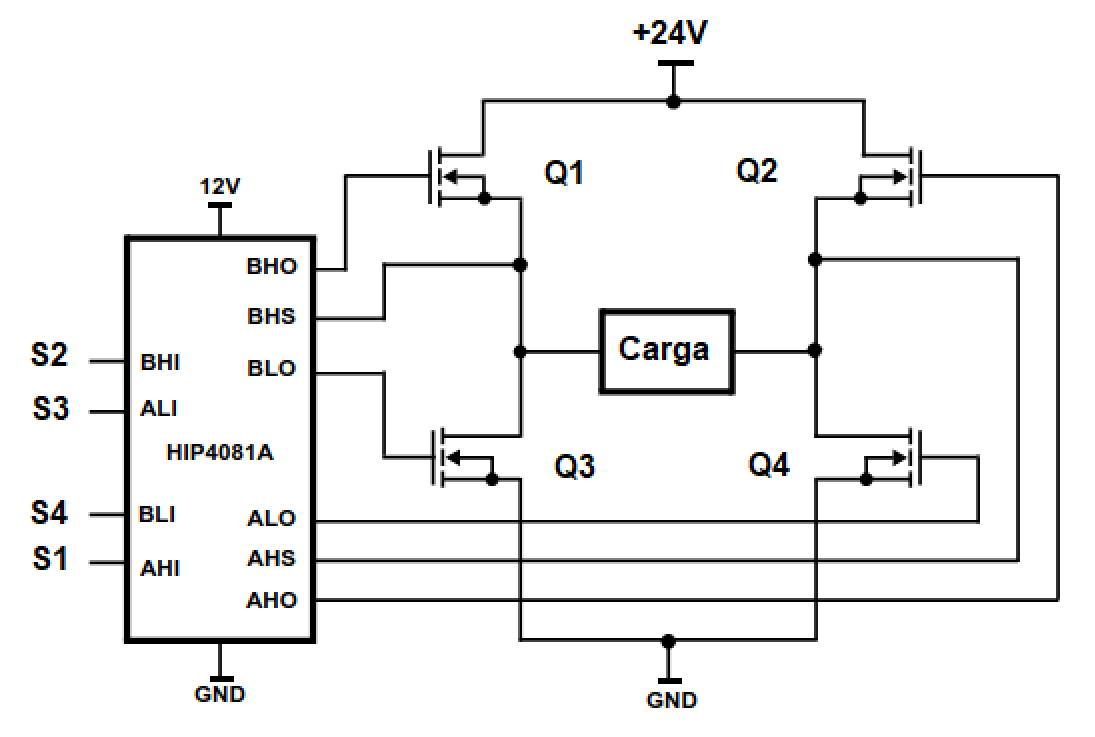
\includegraphics[scale=0.7]{Topologia-puenteH.png}
	\caption{Topología elemental del puente H.}
	\label{fig:img_topologia-puenteH}
\end{figure}
